\section{Calibration Script}

An important step when dealing with accelerometer and gyroscope data is taking care of axes alignment. For example, if the application involves installation of the sensors system on a car, it is important for the boards to be positioned in a coherent way: all the sensor chips have their own axes orientation, and it's a good idea to align them to the vehicle ones. 

A problem may arise if the final user puts the sensors in a wrong way, rotated with respect to the desired direction. In this case, the obtained data should be post-processed accordingly, to get reasonable results: in particular, a rotation matrix should be calculated and then multiplied to the raw acceleration data. 



I had at my disposal an algorithm, wirtten for MATLAB, able to calculate the roll, pitch and yaw angles, developed by the research group I'm working with for this thesis (Electronic Design Automation Group) and optimized for embedded systems application: this algorithm iterates over GPS and IMU data, performing two kinds of calibration, explained as follows.
\begin{itemize}
    \item \textbf{Static Calibration}. Working on a subset of samples, the available data is analyzed to verify if the vehicle the sensor is mounted on is static. If this is the case, the subset of samples is passed to a dedicated procedure able to extract two angles: alpha (roll) and gamma (pitch). 
    \item \textbf{Dynamic Calibration}. Also in this case a subset of samples is analyzed, but here the algorithm verifies if the vehicle is proceeding in a straight path. This step is necessary because, if that condition is met, the buffer of samples undergoing this condition is elaborated, along with the alpha and gamma angles: the output is the beta (yaw) angle. 
\end{itemize}

Once the three angles have been calculated, it is possible to generate the three rotation matrices to be applied to the motion data \(m_{\alpha} , m_{\beta} , m_{\gamma}\) as represented in Equations \ref{m-alpha}, \ref{m-beta} and \ref{m-gamma}. The goal, given the reference system \(R_S\) of the IMU sensors, is to achieve the alignment with the reference system \(R_M\) of the vehicle, as explained in Figure \ref{fig:reference-systems}.

    \begin{figure}[ht!]
        \centering
        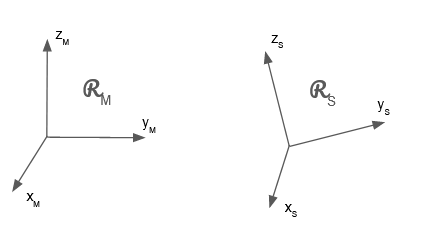
\includegraphics[width=0.5\textwidth]{chap3/figure/calibration_algo_axes.png}
        \caption{Example of sensors reference system compared to vehicle reference system. }
        \label{fig:reference-systems}
    \end{figure}

\begin{equation} \label{m-alpha}
m_{\alpha} = \begin{bmatrix}
    cos(\alpha)     & 0     & sin(\alpha)       \\
    0               & 1     & 0                 \\
    -sin(\alpha)    & 0     & cos(\alpha)       \\
\end{bmatrix}
\end{equation}


\begin{equation} \label{m-beta}
m_{\beta} = \begin{bmatrix}
    cos(\beta)      & -sin(\beta)     & 0       \\
    sin(\beta)      & cos(\beta)      & 0       \\
    0               & 0               & 1       \\
\end{bmatrix}
\end{equation}

\begin{equation} \label{m-gamma}
m_{\gamma} = \begin{bmatrix}
    1      & 0     & 0       \\
    0      & cos(\gamma)      & -sin(\gamma)       \\
    0               & sin(\gamma)               & cos(\gamma)      \\
\end{bmatrix}
\end{equation}

The system I'm working on does not include any GPS sensor, hence this algorithm required some modifications in order to be useful. In particular, I modified the two functions that are responsible of recognizing the static and dynamic conditions, generating the corresponding sample subsets. In the new version of the script, these functions are no more accepting GPS data as inputs, and they verify (a) the static condition by checking if the variance of both acceleration and gyroscope samples is below a certain threshold and (b) the dynamic condition by calculating the variance of the gyroscope samples and comparing it to a threshold. Then, the calculation of the angles remains as before, because that step requires the IMU samples only. Some work was necessary to correctly fix the thresholds for the variance values, that have been decreased from the original values to reach more precise results in calibration. 

In Figure \ref{fig:calibration-flow} the flowchart of the algorithm is reported. The two different kind of calibration are reported in different colors. 

It is evident that the calibration is performed in an iterative way, by repeating the static and dynamic calibration over different chunks of samples (moving the \textit{start} index). Each cycle will generate different values for the angles, and at the end the median value is calculated and shown as output.
The two calibration procedures will take the sample corresponding to the \textit{start} index, and then add values (one second of samples per cycle) until the variance of the buffer overcomes the threshold value. In this case, the last second of samples is flushed (because the condition is no more met), and, if the remaining ones represent the static/dynamic condition for at least a certain number of seconds, those IMU samples are used to perform calculation of the required angles (alpha and gamma for static, beta for dynamic). 

    \begin{figure}[ht!]
        \centering
        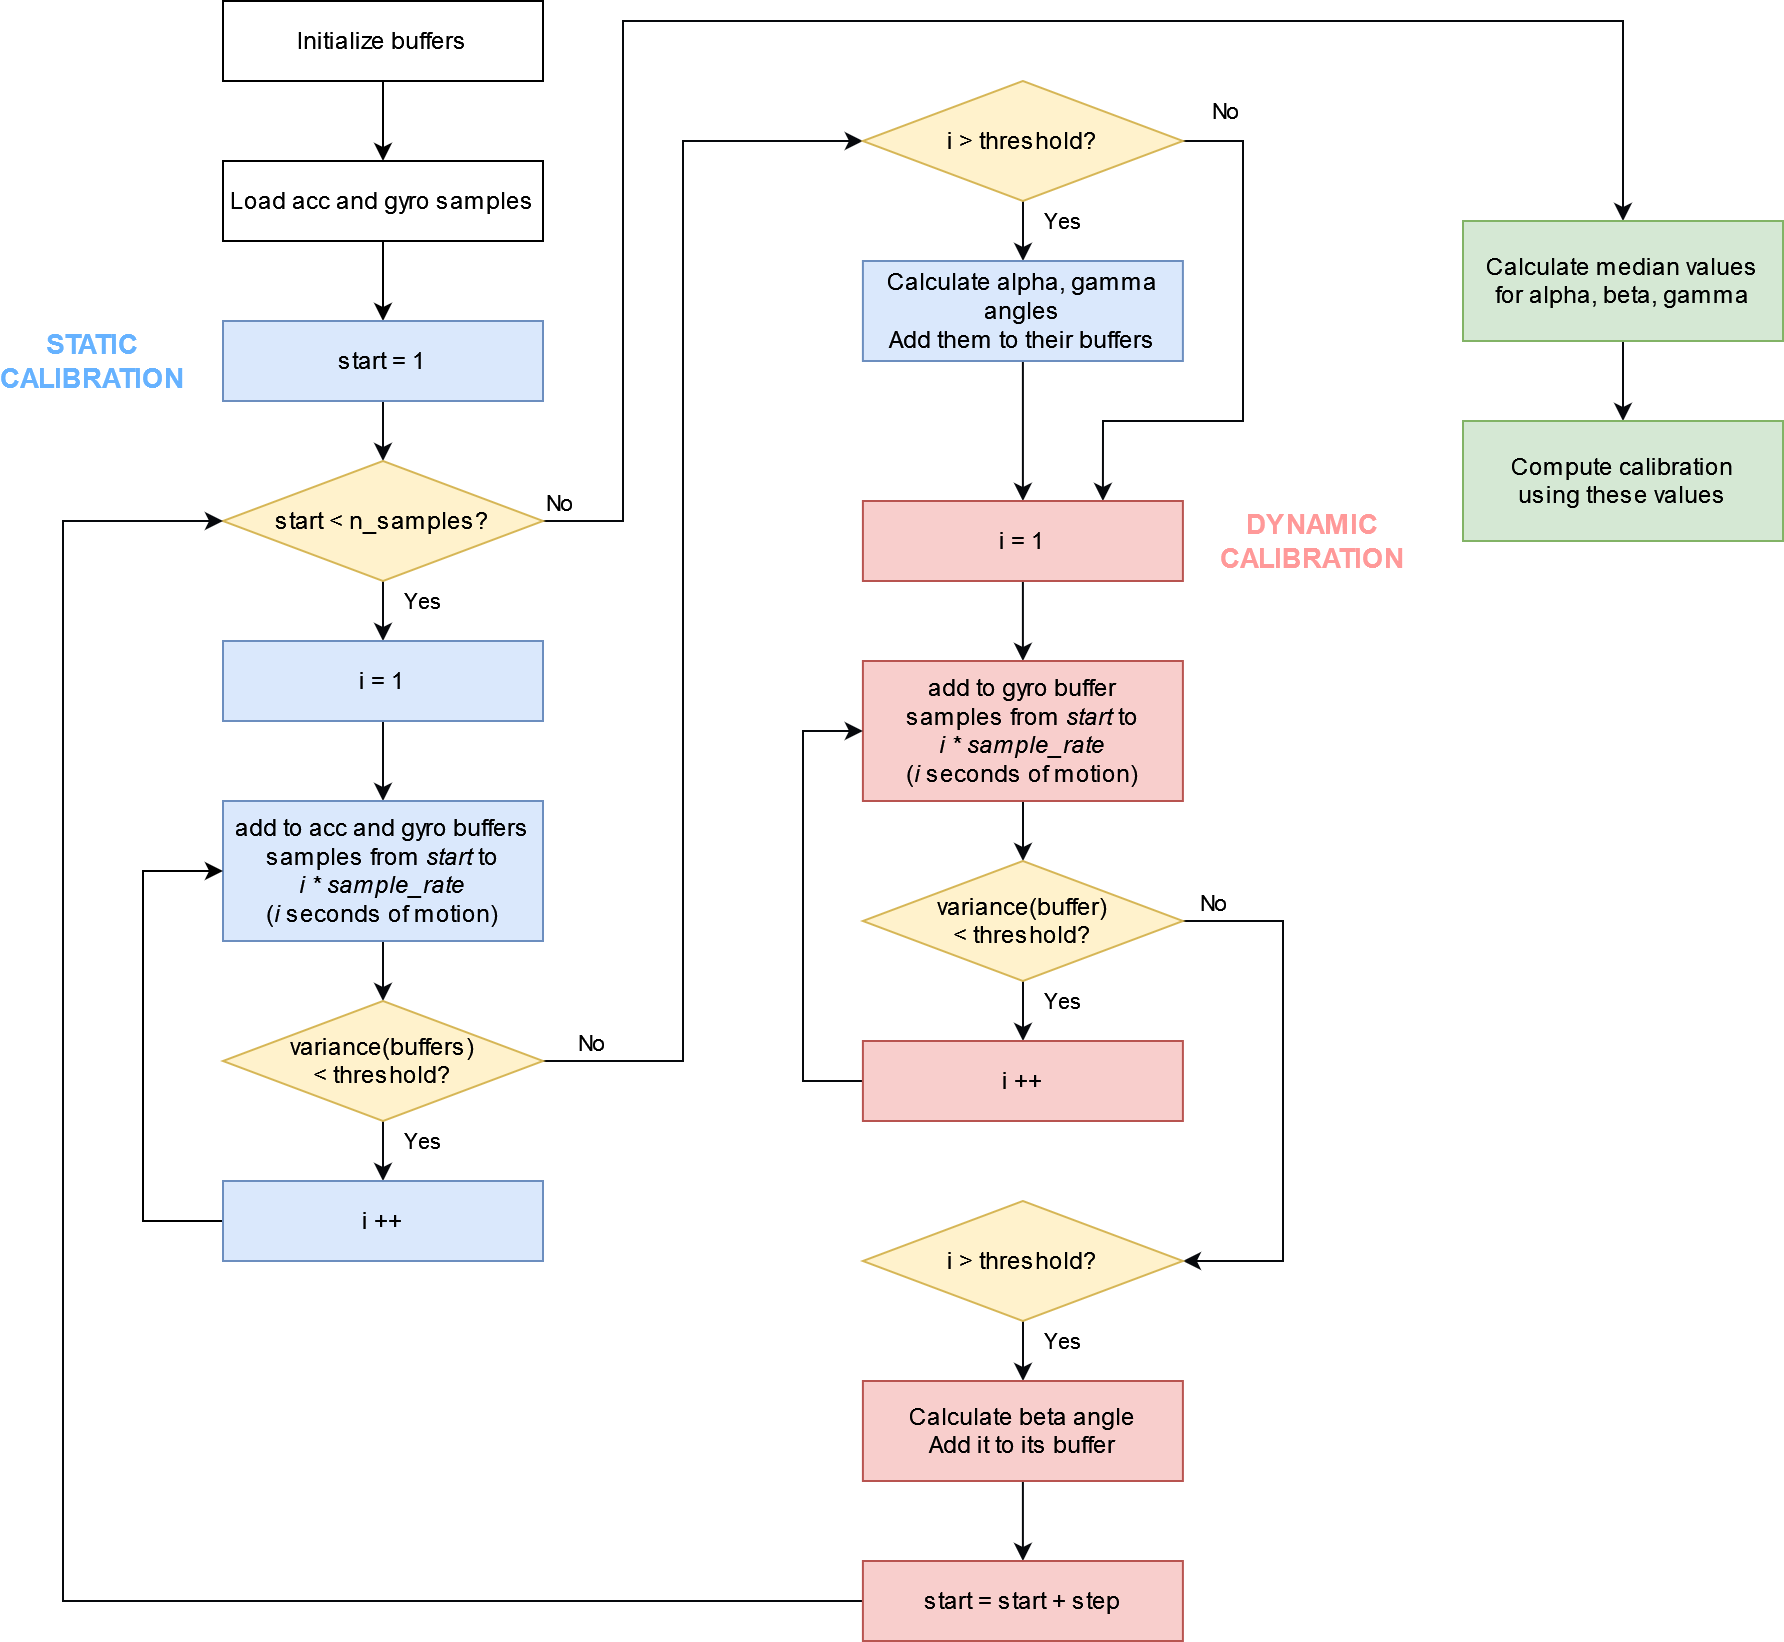
\includegraphics[width=\textwidth]{chap3/figure/calibration_flowchart.png}
        \caption{Flowchart of the script that perform calibration of the axes.}
        \label{fig:calibration-flow}
    \end{figure}

\clearpage